We can rearrange the Friedman equations into
\begin{gather}
    \ins{\frac{\dot{R}}{R}}^2 = \frac{8\pi}{3}G\rho - \frac{Kc^2}{R^2} \\
    \frac{\ddot{R}}{R} = -\frac{4\pi G}{3c^2}\ins{\rho c^2 + 3P}
\end{gather}
We'll investigate these equations: in a a static universe \(\dot{R} = 0\) and \(\ddot{R} = 0\) and if we plug that into the 2nd equation, where pressure and density must be non-negative, the only solution is an empty universe with no density and no pressure. By the way, this troubled Einstein so much that he added a cosmological constant to his equations to allow for a static universe. We'll add it later. Leaving this scenario behind, the 2nd equation says that for a non-empty universe the expansion must be decelerating: \(\ddot{R} < 0\). Observations show that the expansion is actually accelerating, so something must be missing from the equation. We're looking at the incomplete equations for pedagogical purposes only. Sometimes it's useful to combine the equations into what's called the third Friedmann equation or the fluid equation:
\begin{equation}
    \dot{\rho}c^2 = -3\frac{\dot{R}}{R} \ins{\rho c^2 + P}
\end{equation}
\begin{wrapfigure}[25]{r}{0.5\textwidth}
    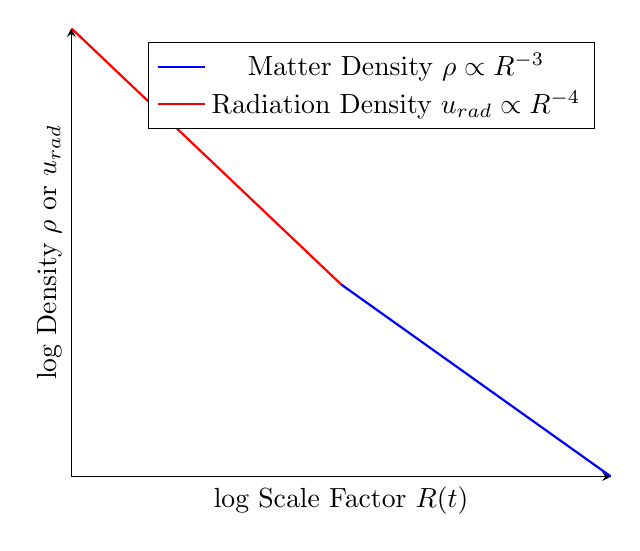
\begin{tikzpicture}
        \begin{axis}[
            xlabel={log Scale Factor \(R(t)\)},
            ylabel={log Density \(\rho\) or \(u_{rad}\)},
            axis lines=left,
            xmode=log,
            ymode=log,
            domain=1:100,
            samples=100,
            legend pos=north east,
            ticks=none
        ]
        \addplot[blue, thick, domain=10:100] {x^(-3)/10};
        \addlegendentry{Matter Density \(\rho \propto R^{-3}\)}
        \addplot[red, thick, domain=1:10] {x^(-4)};
        \addlegendentry{Radiation Density \(u_{rad} \propto R^{-4}\)}
        \end{axis}
    \end{tikzpicture}
    \caption{Density as a function of scale factor, showing the difference between matter and radiation domination. It can be shown that \(a = \frac{R}{R_0} = \frac{1}{3500}\) and \(\frac{t}{t_0} = \frac{1}{\qty{2e5}{unit}}.\)}
    \label{fig:density_radius}
\end{wrapfigure}
this equation can also be reached using thermodynamics. Our goal now is to find an expression for \(R(t)\). We'll look at different ages of the universe. In the matter dominated era, radiation pressure is negligible compared to energy density, so \(P \ll \rho c^2\). The fluid equation becomes
\begin{equation}
    \frac{\dot{\rho}}{\rho} = -3\frac{\dot{R}}{R}
\end{equation}
which is a simple differential equation with solution
\begin{equation}
    \rho(t) \propto R(t)^{-3}
\end{equation}
in the radiation dominated era, we'll replace the element \(\rho c^2\) with \(u_{rad}\) and earlier in the course we found that \(P = u_{rad}/3\). The fluid equation becomes
\begin{equation}
    \dot{u}_{rad} = -3\frac{\dot{R}}{R} \ins{u_{rad}+\frac{1}{3}u_{rad}} = -4\frac{\dot{R}}{R}u_{rad}
\end{equation}
with solution
\begin{equation}
    u_{rad}(t) \propto R(t)^{-4}
\end{equation}
we can then find that in the radiation dominated era, \(R \propto t^{1/2}\) and in the matter dominated era, \(R \propto t^{2/3}\). In late times the element \(K\frac{c^2}{r^2}\) becomes important, this is called the curvature dominated era. We'll look at the three possibilities for \(K\). If \(K=0\) (the flat universe) then from the first Friedmann equation we have
\begin{equation}
    \frac{\dot{R}}{R} = H^2 = \sqrt{\frac{8\pi G \rho}{3}}
\end{equation}
from observations we know \(H_0 = \frac{8\pi G}{3}\rho_0\). We define a critical density as
\begin{equation}
    \rho_c = \frac{3H^2}{8\pi G}
\end{equation}
inserting current values we find \(\rho_c = \qty{1.4e11}{}\frac{M_\mathSun}{\qty{}{\mega\parsec^3}}\). We can then define a density parameter as
\begin{equation}
    \Omega = \frac{\rho}{\rho_c}
\end{equation}
if \(\Omega = 1\) the universe is flat, if \(\Omega > 1\) the universe is closed, and if \(\Omega < 1\) the universe is open. Continuing to the case \(K=1\), the closed universe, we have
\begin{equation}
    \ins{\frac{\dot{R}}{R}}^2 = \frac{8\pi G}{3}\rho - \frac{c^2}{R^2}
\end{equation}
The two elements on the right hand side will eventually balance out, at which point \(\dot{R} = 0\) and the universe stops expanding and starts contracting. The maximum radius can be found by setting the right hand side to zero:
\begin{equation}
    R_{max} = \sqrt{\frac{3c^2}{8\pi G \rho}}
\end{equation}
In the case \(K=-1\), the open universe, 
\begin{equation}
    \ins{\frac{\dot{R}}{R}}^2 = \frac{8\pi G}{3}\rho + \frac{c^2}{R^2}
\end{equation}
and in large times \(\dot{R} \rightarrow c\). Overall if we graph \(R(t)\) for the three cases we get something like this:
% figure
Another way of writing the Friedmann equations is by defining \(\Omega_{m,o} = \frac{\rho_{m,0}}{\rho_{c,0}}\), \(\Omega_{rad,0} =  \frac{\rho_{rad,0}}{\rho_{c,0}}\), \(\Omega_0 = \sum\Omega_{i,0}\), \(a=\frac{R}{R_0}\), and \(H = \frac{\dot{R}}{R}\). The first Friedmann equation becomes
\begin{equation}
    \ins{\frac{H}{H_0}}^2 = \frac{\Omega_{m,0}}{a^3} + \frac{\Omega_{rad,0}}{a^4} + \frac{1-\Omega_0}{a^2}
\end{equation}
In the case of a flat universe, \(\Omega_0 = 1\) and the last term vanishes. If \(K=1\) then \(\Omega_0 > 1\) and if \(K=-1\) then \(\Omega_0 < 1\). In the general case we can find \(a(t)\) from this equation using \(H = \frac{\dot{a}}{a}\) and solving the differential equation. For example, let's find the age of the universe today by solving for a flat universe. We'll ignore the radiation term since it's negligible today. We're left with
\begin{equation}
    \ins{\frac{\dot{a}}{a}}^2 = H_0^2 \frac{\Omega_{m,0}}{a^3}
\end{equation}
Since \(\Omega_{m,0}\) is the only contributor to \(\Omega_0\) in this scenario, it must be equal to 1. Rearranging and integrating we get
\begin{equation}
    \int\limits_0^{t_0} H_0 \dl t = H_0 t_0 = \int\limits_0^1 \ins{\frac{1}{a^3}}^{-1/2} \dl a = \frac{2}{3}
\end{equation}
therefore
\begin{equation}
    t_0 = \frac{2}{3H_0}
\end{equation}
which is about \(\qty{9}{\giga\year}\). This is lower than the actual age of the universe, about \(\qty{13.8}{\giga\year}\), because we ignored dark energy which is causing the expansion to accelerate. Back to Einstein's issue with the friedmann equations predicting a non-static universe, he added a cosmological constant \(\Lambda\) to the equations:
\begin{gather}
    \ins{\frac{\dot{R}}{R}}^2 = \frac{8\pi G}{3}\rho - \frac{Kc^2}{R^2} + \frac{1}{3}\Lambda \\
    \frac{\ddot{R}}{R} = -\frac{4\pi G}{3c^2}\ins{\rho c^2 + 3P} + \frac{1}{3}\Lambda \\
    \dot{\rho}c^2 = -3\frac{\dot{R}}{R}\ins{\rho c^2 + P}
\end{gather}
Later observations by hubble showed that the universe is expanding, so Einstein called the addition of the cosmological constant his `biggest mistake'. Recent observations however show that the expansion is accelerating, so the cosmological constant (or something like it) is used again, with the interpretation that it represents dark energy. We can see that if \(\Lambda\) is large enough, the 2nd equation can give \(\ddot{R} > 0\). If we define the dark energy density as
\begin{equation}
    \rho_\Lambda = \frac{\Lambda}{8\pi G}
\end{equation}
and the dark energy density as
\begin{equation}
    \epsilon_\Lambda = \rho_\Lambda c^2 = \frac{\Lambda c^2}{8\pi G}
\end{equation}
and 
\begin{equation}
    \Omega_\Lambda = \frac{\rho_\Lambda}{\rho_c} = \frac{\Lambda}{3H^2}
\end{equation}
we can rewrite the first Friedmann equation as
\begin{equation}
    \ins{\frac{H}{H_0}}^2 = \frac{\Omega_{m,0}}{a^3} + \frac{\Omega_{rad,0}}{a^4} + \Omega_{\Lambda} + \frac{1-\Omega_0}{a^2}
\end{equation}
We can see that since \(\Lambda\) is constant, so is the energy density \(\epsilon_\Lambda\). Let's look into this oddity. The state equation is
\begin{equation}
    \dot{\epsilon} = -3\frac{\dot{R}}{R}\ins{\epsilon + P}
\end{equation}
if we define \(\omega = \frac{P}{\epsilon}\) then
\begin{equation}
    \frac{\dot{\epsilon}}{\epsilon} = -3\frac{\dot{R}}{R}\ins{1+\omega}
\end{equation}
for non-relativistic matter \(P \ll \rho c^2\) which gives \(\omega \simeq 0\). For relativistic matter or radiation we get \(\omega = 1/3\). For dark energy we want \(\dot{\epsilon} = 0\) which gives \(\omega = -1\). A theory that was proposed for the constant energy density is that of vacuum energy. In quantum field theory the vacuum has an energy associated with it, and this energy density is constant as space expands. This is given by
\begin{equation}
    \epsilon_{vac} = \frac{E_P}{l_P^3} = \qty{3e127}{\electronvolt\per\centi\meter\cubed}
\end{equation}
but observations give
\begin{equation}
    \epsilon_\Lambda \approx \qty{4000}{\electronvolt\per\centi\meter\cubed}
\end{equation}
which is a huge discrepancy. This is called the cosmological constant problem and is an open question in physics. Expansion with the cosmological constant becomes dominant at late times, when the matter and radiation densities have dropped enough.
\begin{equation}
    H^2 = \ins{\frac{\dot{R}}{R}}^2 = \frac{1}{3}\Lambda
\end{equation}
which has solution
\begin{equation}
    R(t) \propto e^{\sqrt{\frac{\Lambda}{3}}t}
\end{equation}